\documentclass[border=4pt]{standalone}
\usepackage{tikz}
\usepackage{pgfplots}
\pgfplotsset{compat=1.18}
\usetikzlibrary{shapes.geometric,arrows.meta,positioning,calc,fit,decorations.pathreplacing,backgrounds}
\definecolor{boxblue}{RGB}{225,238,252}
\definecolor{boxgreen}{RGB}{225,247,231}
\definecolor{boxorange}{RGB}{253,236,216}
\definecolor{boxgray}{RGB}{237,237,237}
\definecolor{boxred}{RGB}{253,226,226}
\begin{document}
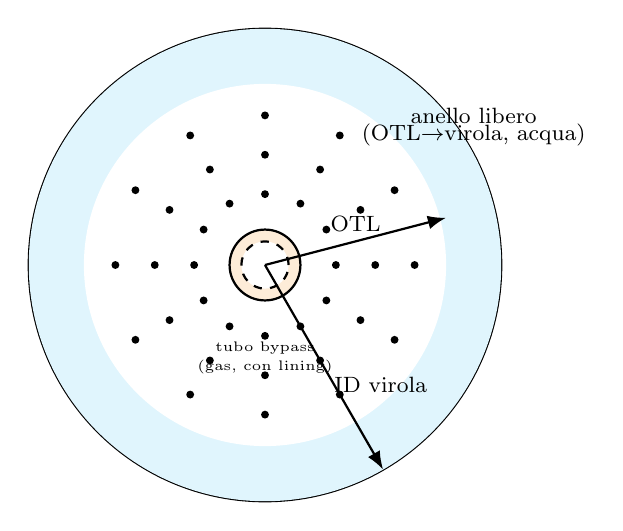
\begin{tikzpicture}[scale=1.0]
\draw[thick] (0,0) circle (3.0);
\draw[dashed,thick] (0,0) circle (2.3);
\fill[cyan!12] (0,0) circle (3.0);
\fill[white] (0,0) circle (2.3);
% tube pattern inside OTL
\foreach \r in {0.4,0.9,1.4,1.9}{
  \foreach \a in {0,30,...,330}{
    \fill[black] ({\r*cos(\a)},{\r*sin(\a)}) circle (0.05);
  }
}
% central bypass tube: GAS-carrying, lined
\fill[boxorange] (0,0) circle (0.45);
\fill[white] (0,0) circle (0.30);
\draw[thick] (0,0) circle (0.45);
\draw[thick,dashed] (0,0) circle (0.30);
\node[font=\tiny] at (0,-1.05) {tubo bypass};
\node[font=\tiny] at (0,-1.3) {(gas, con lining)};
\node[font=\footnotesize] at (2.65,1.9) {anello libero};
\node[font=\footnotesize] at (2.65,1.65) {(OTL$\to$virola, acqua)};
\draw[-{Latex},thick] (0,0) -- (2.3,0.6) node[midway,above,font=\footnotesize]{OTL};
\draw[-{Latex},thick] (0,0) -- ({3.0*cos(-60)},{3.0*sin(-60)}) node[midway,below right,font=\footnotesize]{ID virola};
\end{tikzpicture}
\end{document}
